\documentclass[a4paper,12pt]{article}
\usepackage[indonesian]{babel}
\usepackage{graphicx}
\usepackage{multirow}
\usepackage{enumitem}
\usepackage{listings}
\usepackage{wrapfig}
\usepackage[T1]{fontenc}
\usepackage{inconsolata}
\usepackage{lipsum}
\usepackage{adjustbox}
\usepackage{upquote}


\usepackage{color}
\usepackage[table]{xcolor}
\definecolor{lightgray}{rgb}{0.95, 0.95, 0.95}
\definecolor{darkgray}{rgb}{0.4, 0.4, 0.4}
%\definecolor{purple}{rgb}{0.65, 0.12, 0.82}
\definecolor{editorGray}{rgb}{0.95, 0.95, 0.95}
\definecolor{editorOcher}{rgb}{1, 0.5, 0} % #FF7F00 -> rgb(239, 169, 0)
\definecolor{editorGreen}{rgb}{0, 0.5, 0} % #007C00 -> rgb(0, 124, 0)
\definecolor{orange}{rgb}{1,0.45,0.13}		
\definecolor{olive}{rgb}{0.17,0.59,0.20}
\definecolor{brown}{rgb}{0.69,0.31,0.31}
\definecolor{purple}{rgb}{0.38,0.18,0.81}
\definecolor{lightblue}{rgb}{0.1,0.57,0.7}
\definecolor{lightred}{rgb}{1,0.4,0.5}
% CSS
\lstdefinelanguage{CSS}{
  keywords={color,background-image:,margin,padding,font,weight,display,position,top,left,right,bottom,list,style,border,size,white,space,min,width, transition:, transform:, transition-property, transition-duration, transition-timing-function},	
  sensitive=true,
  morecomment=[l]{//},
  morecomment=[s]{/*}{*/},
  morestring=[b]',
  morestring=[b]",
  alsoletter={:},
  alsodigit={-}
}

% JavaScript
\lstdefinelanguage{JavaScript}{
  morekeywords={typeof, new, true, false, catch, function, return, null, catch, switch, var, if, in, while, do, else, case, break},
  morecomment=[s]{/*}{*/},
  morecomment=[l]//,
  morestring=[b]",
  morestring=[b]'
}

\lstdefinelanguage{HTML5}{
  language=html,
  sensitive=true,	
  alsoletter={<>=-},	
  morecomment=[s]{<!-}{-->},
  tag=[s],
  otherkeywords={
  % General
  >,
  % Standard tags
	<!DOCTYPE,
  </html, <html, <head, <title, </title, <style, </style, <link, </head, <meta, />,
	% body
	</body, <body,
	% Divs
	</div, <div, </div>, 
	% Paragraphs
	</p, <p, </p>,
	% scripts
	</script, <script,
  % More tags...
  <canvas, /canvas>, <svg, <rect, <animateTransform, </rect>, </svg>, <video, <source, <iframe, </iframe>, </video>, <image, </image>, <header, </header, <article, </article
  },
  ndkeywords={
  % General
  =,
  % HTML attributes
  charset=, src=, id=, width=, height=, style=, type=, rel=, href=,
  % SVG attributes
  fill=, attributeName=, begin=, dur=, from=, to=, poster=, controls=, x=, y=, repeatCount=, xlink:href=,
  % properties
  margin:, padding:, background-image:, border:, top:, left:, position:, width:, height:, margin-top:, margin-bottom:, font-size:, line-height:,
	% CSS3 properties
  transform:, -moz-transform:, -webkit-transform:,
  animation:, -webkit-animation:,
  transition:,  transition-duration:, transition-property:, transition-timing-function:,
  }
}

\lstdefinestyle{htmlcssjs} {%
  % General design
%  backgroundcolor=\color{editorGray},
  basicstyle={\footnotesize\ttfamily},   
  frame=single,
  % line-numbers
  % Code design
  identifierstyle=\color{black},
  keywordstyle=\color{blue}\bfseries,
  ndkeywordstyle=\color{editorGreen}\bfseries,
  stringstyle=\color{editorOcher}\ttfamily,
  commentstyle=\color{brown}\ttfamily,
  % Code
  language=HTML5,
  alsolanguage=JavaScript,
  alsodigit={.:;},	
  tabsize=2,
  showtabs=false,
  showspaces=false,
  showstringspaces=false,
  extendedchars=true,
  breaklines=true,
  % German umlauts
  literate=%
  {Ö}{{\"O}}1
  {Ä}{{\"A}}1
  {Ü}{{\"U}}1
  {ß}{{\ss}}1
  {ü}{{\"u}}1
  {ä}{{\"a}}1
  {ö}{{\"o}}1
}
%
\lstdefinestyle{py} {%
language=python,
literate=%
*{0}{{{\color{lightred}0}}}1
{1}{{{\color{lightred}1}}}1
{2}{{{\color{lightred}2}}}1
{3}{{{\color{lightred}3}}}1
{4}{{{\color{lightred}4}}}1
{5}{{{\color{lightred}5}}}1
{6}{{{\color{lightred}6}}}1
{7}{{{\color{lightred}7}}}1
{8}{{{\color{lightred}8}}}1
{9}{{{\color{lightred}9}}}1,
basicstyle=\footnotesize\ttfamily, % Standardschrift
numbers=left,               % Ort der Zeilennummern
%numberstyle=\tiny,          % Stil der Zeilennummern
%stepnumber=2,               % Abstand zwischen den Zeilennummern
numbersep=5pt,              % Abstand der Nummern zum Text
tabsize=4,                  % Groesse von Tabs
extendedchars=true,         %
breaklines=true,            % Zeilen werden Umgebrochen
keywordstyle=\color{blue}\bfseries,
frame=b,
commentstyle=\color{brown}\itshape,
stringstyle=\color{editorOcher}\ttfamily, % Farbe der String
showspaces=false,           % Leerzeichen anzeigen ?
showtabs=false,             % Tabs anzeigen ?
xleftmargin=17pt,
framexleftmargin=17pt,
framexrightmargin=5pt,
framexbottommargin=4pt,
%backgroundcolor=\color{lightgray},
showstringspaces=false,      % Leerzeichen in Strings anzeigen ?
}%
%
\definecolor{dkgreen}{rgb}{0,.6,0}
\definecolor{dkblue}{rgb}{0,0,.6}
\definecolor{dkyellow}{cmyk}{0,0,.8,.3}

\lstdefinestyle{PHP}{
  language        = php,
  basicstyle      = \small\ttfamily,
  keywordstyle    = \color{dkblue},
  stringstyle     = \color{red},
  identifierstyle = \color{dkgreen},
  commentstyle    = \color{gray},
  emph            =[1]{php},
  emphstyle       =[1]\color{black},
  emph            =[2]{if,and,or,else},
  emphstyle       =[2]\color{dkyellow}}
\lstset{
    showstringspaces=false,
    frame=single,
    breaklines=true,
    rulecolor=\color{black},
    style=htmlcssjs
}
%

\graphicspath{ {./img/} }
\begin{document}
\title{ {\Large Laporan Praktikum}\\ Pemrograman Web Client\\{\Large Pertemuan 11}}

\author{Aldzikri Dwijayanto Prathama 
	\\195410189
	\\Informatika}
\makeatletter
\begin{titlepage}
	\begin{center}
		{\huge \bfseries \@title }\\[14ex]
		
\includegraphics[scale=.8]{logo}\\[4ex]
		{\large \@author}\\[12ex]
		{\large \bfseries {SEKOLAH TINGGI MANAJEMEN INFORMATIKA DAN KOMPUTER
				AKAKOM YOGYAKARTA}}
	\end{center}


%{\large \@date} 
\end{titlepage}
\makeatother
%\maketitle
\renewcommand{\figurename}{Gambar}
\newpage
\tableofcontents
\newpage
\section{Tujuan}
Mahasiswa mampu menuliskan script javascript untuk membuat web dinamis menggunakan DOM.\@ Dan mampu menuliskan script untuk validasi form.
\section{Dasar Teori}

DOM atau document object model adalah standar objek Model dan pemrograman antarmuka untuk HTML.\@ Dalam kata lain, DOM
adalah standar untuk melakukan bagaimana mendapatkan, merubah, menambah, dan menghapus HTML.\@\\

Validasi Form adalah suatu cara untuk menghindari kesalahan dalam mengisi field pada suatu form dengan menampilkan alert
dan memberikan nilai balik false agar form tidak dikirim. Sebagai contoh jika suatu field pada form belum terisi maka
javascript akan menampilkan alert bahwa field tersebut belum terisi.

\newpage

\section{Pembahasan}
\subsection{Praktik}
\subsubsection{Praktik 1}
\textbf{DOM Methods\\}
\begin{lstlisting}[style=htmlcssjs]
<!DOCTYPE html>
<html>
    <body>
        <h2>My First Page</h2>
        <p id="demo"></p>

   <script>
       document.getElementById("demo").innerHTML = "Hello World!";
   </script>

    </body>
</html>
\end{lstlisting}
Pada praktik 1, adalah menampilkan tulisan dengan dom method. Pada elemen <p> diberi id demo. Kemudian pada script,
digunakan document, lalu dengan getElementById, javascript akan merubah elemen yang memiliki id demo, dengan mengisikan
kalimat ``Hello World''.
\begin{center}
    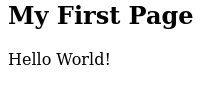
\includegraphics[scale=.7]{1.png} 
\end{center}

\subsubsection{Praktik 2}
\textbf{DOM Elements}
\begin{lstlisting}
<!DOCTYPE html>
<html>
    <body>
        <h2>Finding HTML Elements by Id</h2>

        <p id="intro">Hello World!</p>
        <p>This example demonstrate the <b>getElementById</b> method.</p>
        <p id="demo"></p>

   <script>
       var myElement = document.getElementById("intro");
       document.getElementById("demo").innerHTML = 
           "The text from the intro paragraph is " + myElement.innerHTML;
   </script>

    </body>
</html>
\end{lstlisting}
Pada Praktik 2 ini kita akan menampilkan output sederhana menggunakan DOM Elements. Bisa dilihat pada baris ke-7 kita
tambahkan tag p dengan atribut id dengan valuenya intro. Kemudian pada baris ke-10 kita tambahkan tag p dengan atribut
id dan valuenya demo. Pada baris ke-12 sampai ke-16 kita tambahkan tag script. Pad baris ke-13 kita tambahkan variabel
myElement dengan valuenya dari objek document untuk membaca elemen html berdasarkan id-nya yaitu intro. Kemudian pada
baris ke-14 kita tambahkan fungsi getElementById() dari objek document untuk membaca elemen html berdasarkan id-nya
yaitu demo.

\begin{center}
    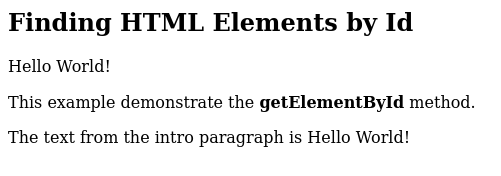
\includegraphics[scale=.7]{2.png} 
\end{center}

\subsubsection{Praktik 3}
\textbf{DOM HTML}
\begin{lstlisting}
<!DOCTYPE html>
<html>
    <body>
   <script>
       document.write(Date());
   </script>
    </body>
</html>

\end{lstlisting}

Untuk praktik selanjutnya dibuat dokumen html, yang memiliki script internal. Script tersebut akan menanmpilkan waktu
pada komputer ke halaman, ketika dibuka di browser.
\begin{center}
    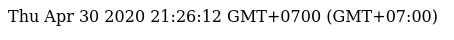
\includegraphics[scale=.7]{3.png} 
\end{center}

\subsubsection{Praktik 4}
\textbf{DOM CSS}
\begin{lstlisting}
<!DOCTYPE html>
<html>
    <body>
        <p id="p1">Hello World!</p>
        <p id="p2">Hello World!</p>

    <script>
        document.getElementById("p2").style.color="blue";
        document.getElementById("p2").style.fontFamily="Arial";
        document.getElementById("p2").style.fontSize="larger";
    </script>

    <p>The paragraph above was changed by a script</p>
    </body>

</html>

</html>
\end{lstlisting}
Untuk praktik 4, adalah membuat dokumen html yang styleny diatus dengan DOM CSS.\@ Pertama dibuat dua elemen p, dengan
isi yang sama, tapi dengan id berbeda, elemen <p> pertama memiliki id p1, sedangkan elemen <p> kedua memiliki id p2.
Selanjutnya pada elemen script terdapat fungsi getElementById() dari objek document untuk membaca elemen html
berdasarkan id-nya yaitu p2 dan style untuk mengubah tampilan dari tulisan tersebut.

\begin{center}
    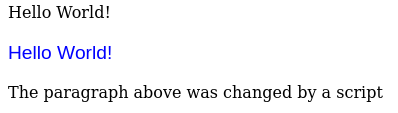
\includegraphics[scale=.7]{4.png} 
\end{center}

\subsubsection{Praktik 5}
\textbf{DOM Events}
\begin{lstlisting}
<!DOCTYPE html>
<html>
    <body>
        <h1 onclick="this.innerHTML='Ooops!'">Click on this text!</h1>
    </body>
</html>
\end{lstlisting}

Praktek senaljutnya adalah membuat laman html, yang akan berubah tulisannya ketika tombol diklik. Untuk membuatnyda
digunakan elemen h1, dengan parameter onclick.

\begin{center}
    
\includegraphics[scale=.7]{5.png} 
\end{center}

\subsubsection{Praktik 6}
\textbf{DOM Event Listener}
\begin{lstlisting}
<!DOCTYPE html>
<html>
    <body>
        <h2>Javascript addEventListener()</h2>
        <p>This example uses the addEventListener() method to attach a click event to a button.</p>
        <button id="myBtn">Try it</button>
        <p id="demo"></p>
        <script>
            document.getElementById("myBtn").addEventListener("click",displayDate);

            function displayDate() {
                document.getElementById("demo").innerHTML=Date();
            }
        </script>
    </body>
</html>
\end{lstlisting}

Pada Praktik 6 ini kita akan menampilkan output sederhana menggunakan DOM Event Listener. Pertama dibuat button terlebih
dahulu dengan menggunakan elemen button. Kemudian kita tambahkan elemen
p dengan atribut id dan valuenya demo. Kemudian pada pada elemen script di dalamnya
terdapat getElementById dari objek document untuk membaca elemen html berdasarkan id-nya yaitu
myBtn dan terdapat addEventListener yang didalamnya terdapat fungsi untuk menampilkan waktu. Kemudian tambahkan fungsi
displayDate yg didalamnya terdapat fungsi untuk menampilkan waktu.

\begin{center}
    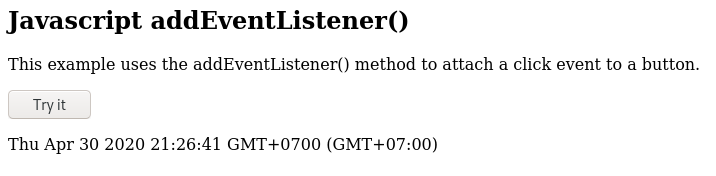
\includegraphics[scale=.7]{6.png} 
\end{center}

\subsubsection{Praktik 7}
\textbf{DOM Navigation}
\begin{lstlisting}
<!DOCTYPE html>
<html>
    <body>
        <h1 id="id01">My First Page</h1>
        <p id="id02"></p>

        <script>
            document.getElementById("id02").innerHTML = document.getElementById("id02").innerHTML;
        </script>
    </body>
</html>
\end{lstlisting}

Pada Praktik 7 ini kita akan menampilkan tampilan sederhana menggunakan DOM Navigation.\@ terdapat elemen h1 dengan
atributnya id dan valuenya id01. Kemudian dibuat element p dengan idnya id02. Pada element script didalamnya terdapat
fungsi getElementById() dari objek document untuk membaca elemen html berdasarkan id-nya yaitu id02 dan didalam html
didambahkan fungsi getElementById() untuk id id01.

\begin{center}
    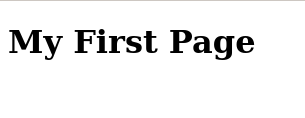
\includegraphics[scale=.7]{7.png} 
\end{center}

\subsubsection{Praktik 8}
\textbf{DOM Nodes}
\begin{lstlisting}
<!DOCTYPE html>
<html>
    <body>
        <div id="div1">
            <p id="p1">This is a paragraph</p>
            <p id="p2">This is another paragraph</p>
        </div>
   <script>
       var para = document.createElement("p");
       var node = document.createTextNode("this id new.");
       para.appendChild(node);
       var element = document.getElementById("div1");
       element.appendChild(para);
   </script>
    </body>
</html>
\end{lstlisting}

Praktik 8 ini kita akan mengetikkan program untuk menampilkan tulisan sederhana menggunakan DOM Node. Pada elemen div
diberi atribut id dan value atributnya div1. Kemudian pada 2 buah baris dibawahnya kita tambahkan tag p dengan id p1
dan p2. Lalu pada elemen script didalamnya terdapat variabel para dengan valuenya createElement pada tag p. Kemudian kita
tambahkan variable node dengan variablenya dengan valuenya createTextNode yang didalamnya akan menampilkan tulisan.
Kemudian pada baris kita tambahkan node untuk var para dengan appendChild.

\subsubsection{Praktik 9}
\textbf{Validasi Form}
\begin{lstlisting}
<!DOCTYPE html>
<html>
    <head>
   <script>
       function validateForm() {
           var x = document.forms["myForm"]["fname"].value;
           if (x == "") {
               alert("Name must be filled out");
               return false;
           }
       }
   </script>
    </head>

    <body>
        <form name="myForm" action="/action_page.php" unsubmit="return validateForm()" method="POST">
		Name: <input type="text" name="fname">
		<input type="submit" value="Submit">
	</form>
	
</body>
</html>
\end{lstlisting}
Praktik 9 ini kita akan mengetikkan program untuk membuat validasi form. Pertama dibuat function validateForm. Kemudian
pada baris berikutnya kita tambahkan variabel x dengan valuenya forms. Dan kemudian kita tambahkan seleksi if. Kemudian
pada baris ke-15 sampai ke-20 kita tambahkan tag body
yang didalamnya terdapat perintah untuk menampilkan inputan Nama dan juga terdapat action untuk proses pada php. Tetapi
pada praktik ini kita tidak membuat file phpnya.

\subsection{Latihan}
\subsubsection{Latihan 1}
\begin{lstlisting}
<!DOCTYPE html>
<html>
<head>
	<script>
		function validateForm()	{
			var x = document.forms["myForm"]["fname"].value;
			var y = document.forms["myForm"]["lalamat"].value;
			var z = document.forms["myForm"]["lemail"].value;
			var a = document.forms["myForm"]["fnotlp"].value;
			var b = document.forms["myForm"]["fjeniskelamin"].value;
			if (x == "" || y == "" || z == "" || a == "" || b == "")  {
				alert("Form must be filled out");
				return false;
			}
		}
	</script>
</head>
<body>

	<form name="myForm" onsubmit="return validateForm()" method="post"> 
		Nama : <input type="text" name="fname">
		Alamat : <input type="text" name="lalamat">
		Email : <input type="text" name="lemail">
		No Telp : <input type="text" name="fnotlp">
		Jenis Kelamin : <input type="text" name="fjeniskelamin">
		<input type="submit" value="Submit">
	</form>
	
</body>
</html>
\end{lstlisting}

Pada latihan ini kita akan membuat Form untuk pendaftaran mahasiswa baru form fieldnya berupa nama, alamat, email, no
telepon, jenis kelamin. Bisa dilihat pada baris ke-5 kita tambahkan function validateForm dengan variabelnya yaitu a
untuk nama, b untuk alamat, c untuk email, i untuk no telp, dan j untuk jenis kelamin. Selanjutnya pada baris ke-11 kita
tambahkan seleksi if dengan tujuan validasi form harus diisi atau tidak boleh kosong. Kemudian pada baris ke-20 sampai
ke-27 kita tambahkan tag form untuk menampilkan inputan Nama, alamat, no telp, email, dan Jenis Kelamin.

\begin{center}
    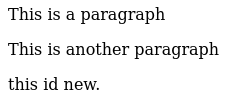
\includegraphics[scale=.7]{8.png} 
\end{center}

\newpage

\section{Kesimpulan}
Setelah praktik mahasiswa mampu menuliskan script javascript untuk membuat web dinamis menggunakan DOM.\@ Dan mampu menuliskan script untuk validasi form.

\end{document}
